\documentclass[a4paper, 12pt]{article}

\usepackage[utf8]{inputenc}
\usepackage[T1]{fontenc}
\usepackage{lmodern}
\usepackage[german]{babel}
\usepackage{helvet}
\renewcommand{\familydefault}{\sfdefault}
\usepackage[singlespacing]{setspace}
\usepackage[margin=1in]{geometry}
\usepackage{parskip}
\usepackage{bibgerm}
\usepackage{graphicx}
\usepackage{tcolorbox}
\usepackage{dingbat}
\usepackage{pdfpages}
\usepackage{hyperref}

\newcommand{\leadingzero}[1]{\ifnum #1<10 0\the#1\else\the#1\fi}
\newcommand{\datumVonHeute}{\leadingzero{\day}.\leadingzero{\month}.\the\year}

\newcommand{\haThema}{"latent-space interpolation"}
\newcommand{\haAutor}{Liza Kaladjian}
\newcommand{\haDeckblattTextEins}{Project in Advances in Intelligent Systems (ISS)}
\newcommand{\haGutachter}{Dr. Dennis Müller}
\newcommand{\haGutachterText}{Professor for Artificial Intelligence and Data Science}

\title{\haThema}
\author{\haAutor}
\date{\today}

\begin{document}

\begin{titlepage}
\noindent
\textbf{Note:} This document was translated by ChatGPT from the original documentation written in German by me.  Original documentation: \href{https://github.com/Lizoug/FaceFusion-Videos-from-Latent-Interpolations/blob/main/German_Documentation/Dokumentation.pdf}{here}.\\
Düsseldorf University of Applied Sciences \\
\begin{center}
\vspace{1.5cm}
{\scshape\large \haDeckblattTextEins \par}
\vspace{1cm}
{\scshape\large on the topic of\par}
\vspace{1.5cm}
{\LARGE\bfseries \haThema \par}
\vfill
{Created by:\\ {\bfseries \haAutor} \par}
\vspace{1cm}
\vspace{1cm}
Supervisor:\\ {\bfseries \haGutachter}\\ \haGutachterText
\vfill
\end{center}
\end{titlepage}
\thispagestyle{empty}
\newpage

\tableofcontents
\thispagestyle{empty}
\newpage

\setcounter{page}{1}

\section{Introduction}
\subsection{Goal and Motivation}
My fascination with Generative Adversarial Networks (GANs) began with my everyday interaction with social media and the Internet. I often encountered impressive applications of GANs without initially understanding the technology behind them. A succinct example that sparked my interest was a challenge on a website where you had to click on the person who was real. This task revealed to me the amazing ability of GANs to produce images so lifelike that they are almost indistinguishable from real photos - a fascinating demonstration of the power of this technology.

These and other applications, such as deepfakes, impressively show how GANs are capable of generating realistic images and videos that are hardly distinguishable from real recordings. One of the most impressive examples that further sparked my curiosity was a \cite{gif_example} that showed a smooth transition between different faces. The ability of GANs to create seamless transitions and transformations inspired me to learn more about this technology and ultimately start a project in this area.

Today, GANs are applied in various fields, from art to the entertainment industry to science. Examples include:
\begin{itemize}
  \item \textbf{Artistic Creations}: Artists use GANs to create unique artworks that often bring forth new perspectives and styles that would not be possible without this technology.\cite{kunstloft_article}
  \item \textbf{Medical Imaging}: In medicine, GANs are used to generate realistic medical images for training purposes without needing to access sensitive patient data.\cite{avinci_ai_gans}
\end{itemize}

These broad applications demonstrate the versatility and transformative potential of GANs. My goal in this project is to develop a deeper understanding of this technology and apply it practically to create my own GIF similar to the GIF example that originally piqued my interest.

\subsection{State of the Art in GANs}
GANs have established themselves as a widespread approach to image synthesis, and this area has seen significant advances through the work of leading organizations like NVIDIA and various research initiatives such as Midjourney. NVIDIA has set new standards in generating hyper-realistic images with its StyleGAN models, particularly StyleGAN2 and StyleGAN3, demonstrating groundbreaking improvements in image quality and consistency, especially known for their ability to generate compelling and consistent facial images.\cite{StyleGAN3, StyleGAN3_Github, StyleGAN2}

The latest model, StyleGAN3, is an improvement over StyleGAN2, introducing key enhancements. For example, StyleGAN3 can better handle camera movements, making it especially useful for video and animation projects.\cite{StyleGAN3_next}

Advancements in 3D GAN technology and the introduction of transformer-based approaches like TransGAN highlight the dynamic and rapidly evolving field of GAN research.\cite{jiang2021transgan} These developments, along with contributions from Midjourney and other research groups, demonstrate the enormous potential of GANs and serve as an important inspiration and benchmark for my own project.

Although I wanted to develop my GAN network from scratch in this project, it was nonetheless fascinating to consider the current state of the art in GANs. I was aware that my simpler models might not achieve the high-grade image quality of the most advanced systems. However, my project focused on gaining a basic understanding of how GANs work. By building and training my model independently, I was able to gain valuable experience and a deep understanding of the complex mechanisms and challenges of GANs. These experiences were enormously valuable to me and enabled me to train a functional model in a relatively short time. This process also showed me how much room for innovation and improvement exists in this

 area and motivated me to continue my research and development in this fascinating field of artificial intelligence.

\subsection{Project Overview}
As mentioned, this project focuses on GANs, specifically on generating and interpolating faces. I used the CelebA dataset from Kaggle, which contains a wide range of faces. This dataset is ideal for training the GANs, as it offers a variety of facial features and expressions and is freely available.\footnote{\url{https://www.kaggle.com/datasets/jessicali9530/celeba-dataset}}

The project consists of two main components:
\begin{enumerate}
  \item \textbf{The Generator (Generator.py)}: This component generates new, realistic facial images based on the CelebA dataset. It's fascinating how the generator creates lifelike images from pure data.
  \item \textbf{The Critic (Critic.py)}: This part evaluates the images created by the generator and helps improve its capabilities by judging how realistic the images are.
\end{enumerate}

An interesting aspect of the project is the \textbf{(Interpolation.py)}, where I experiment with smooth transitions between different faces. The training process, implemented in \textbf{(Trainloop.py)}, uses the CelebA dataset to train both the generator and the critic. The \textbf{(Dataset.py)} supports efficient data handling.

Finally, there's the \textbf{(evaluate\_models.py)}, which serves to assess the quality of the generated images. This helps me judge the progress and performance of the system.

My goal is to develop a deep understanding of GANs and create my own impressive GIF inspired by the applications that led me to this project.

\section{Theoretical Background}
\subsection{Introduction to Generative Adversarial Networks (GANs)}
GAN is a machine learning model where data can be generated using two competing artificial neural networks.\cite{youtube_gans}

One is tasked with generating data that looks real, the other classifies the data as real or artificial. Through continuous learning and many iteration steps, the generated data gets progressively better.\cite{youtube_gans}

The generator creates data, which the discriminator checks against real data. The two networks are logically and mathematically linked in such a way that the data generated by the generator becomes increasingly real. The goal of the generator is to produce data that the discriminator can no longer distinguish from real data.\cite{youtube_gans}

In many iteration steps, the generated data gets better and more closely resembles real data.

\subsection{Problems with Traditional GANs and Solutions through WGANs}
Generative Adversarial Networks (GANs) have revolutionized how we use machine learning for data generation. However, traditional GANs come with several challenges. A central issue is that the discriminator sometimes learns too quickly, giving the generator no chance to improve. This leads to the generator not receiving useful feedback from the discriminator, thus limiting its ability to generate a variety of data.\cite{mathworks_gan_training}

Another problem is the so-called "Mode Collapse"\cite{mathworks_gan_training}. Here, the generator keeps producing the same or very similar images instead of a variety of data. This occurs when the generator finds a simple method to fool the discriminator and then sees no need to vary or improve this method.

\subsection{Wasserstein GANs (WGANs)}
Wasserstein GANs (WGANs) offer solutions to these challenges.\cite{ar5iv_dynamic_discriminator}\cite{ar5iv_contrastive_discriminator} WGANs replace the traditional discriminator with a critic. This critic gives a continuous evaluation instead of a simple real-or-fake classification, leading to more differentiated feedback to the generator. This approach allows the generator to make finer adjustments and generate a greater variety of data.

The Wasserstein loss function used in WGANs helps to optimize the balance between the generator and critic. This function measures the effective distance between the generated and real data, achieving a more stable and meaningful convergence during training.

\section{Project Development}
\subsection{Data Preparation and Processing}

For my project, I used the CelebA dataset available on Kaggle. This dataset is particularly suitable for projects in facial recognition and analysis of facial features. It comprises 202,599 images of various celebrities, divided into 10,177 unique identities, and each image is annotated with 40 binary attribute annotations and 5 landmark positions.

\subsubsection{Data Preparation and Visualization}
Preparing the CelebA dataset for training my GAN model was a crucial step. I developed a Python class `CelebADataset` for processing and loading the images from the dataset.

To process the data efficiently, I implemented a `DataLoader` in PyTorch, which performed several key functions:

\begin{enumerate}
 \item \textbf{Batch processing}: The `DataLoader` loaded the data in batches of 32 images each. This batch processing is essential for training deep neural networks, as it enhances the efficiency of the learning process and optimizes memory usage.

 \item \textbf{Shuffling}: To improve the model's generalization ability and prevent overfitting, the data was shuffled randomly in each epoch. This ensures that the model does not become dependent on the order of the images.

 \item \textbf{Transformations}: The images were first scaled to a uniform size (initially 64x64). Then, a normalization of the image pixels to values between -1 and 1 was performed to ensure consistent input for the neural network.

 \item \textbf{Visualization}: To illustrate the data quality and variety, I generated a sample of images from the DataLoader. These were displayed in a 3x5 grid to provide insight into the different faces and expressions in the CelebA dataset. This visualization was not only important for verifying data quality but also provided information on the diversity of facial features and expressions in the dataset.
\end{enumerate}

\begin{figure}[ht]
\centering
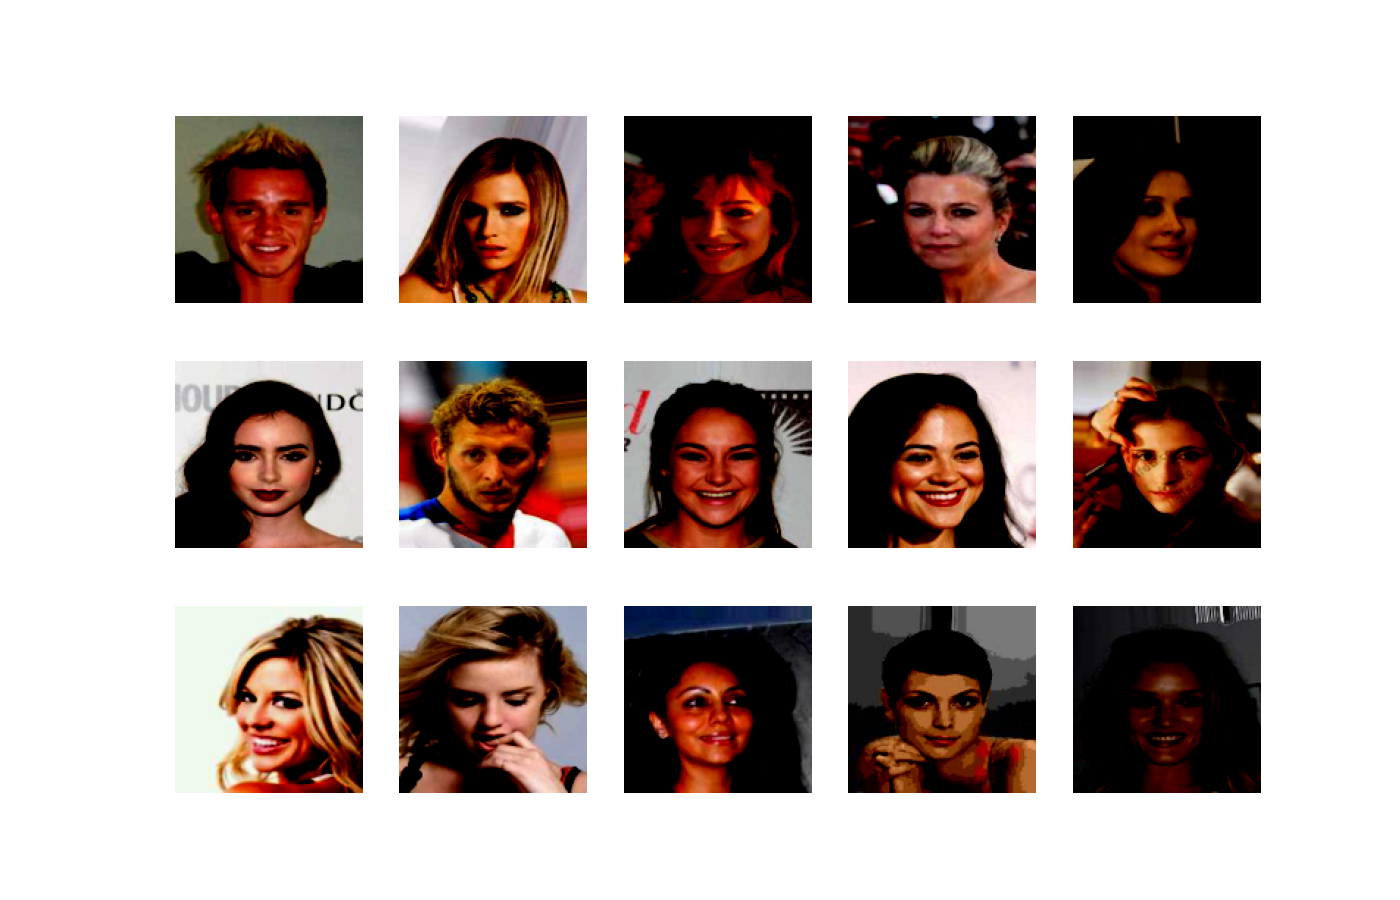
\includegraphics[width=0.8\textwidth]{./img/data_faces.png}
\caption{15 random images from the dataset}
\label{fig:random_faces}
\end{figure}

These steps formed a fundamental basis for efficiently training my GAN model and helped demonstrate the variety and quality of the images used for generating realistic and diverse facial images.

This thorough preparation and review of the CelebA dataset were crucial for gaining a comprehensive overview of the available data \ref{fig:random_faces}. After this meticulous preparation, the data was optimally prepared and ready for the training process of my WGAN model.

\subsection{Construction of the WGAN Architecture}

In this project, I developed a Wasserstein Generative Adversarial Network (WGAN) architecture consisting of two main components: a critic (Critic) and a generator.

\subsubsection{Critic (Critic)}

The critic is a neural network trained to evaluate the images created by the generator. It consists of several layers:

\begin{enumerate}
    \item \textbf{Convolutional layers}: These layers filter features from the input images. I used a total of five convolutional layers, with each layer halving the image resolution and deepening the feature map.
    \item \textbf{Batch normalization}: These layers help improve the stability of the training by normalizing the outputs of the convolutional layers.
    \item \textbf{Leaky ReLU activation}: After each convolutional layer, I use the Leaky ReLU activation function.
   

 \item \textbf{Fully connected layer}: At the end, there is a fully connected layer that converts the features into a single number, representing the critic's evaluation.
\end{enumerate}

\subsubsection{Generator}

The generator is responsible for creating new images. It consists of:

\begin{enumerate}
    \item \textbf{Linear layer}: This layer transforms the input latent vector into a suitable form.
    \item \textbf{Transposed convolutional layers}: Five such layers gradually enlarge the feature map to the target size of the generated images. They are the opposite of normal convolutional layers.
    \item \textbf{Batch normalization and ReLU activation}: Normalizes the output of each layer to stabilize and accelerate the training. It helps to prevent issues like gradient vanishing or exploding.
    \item \textbf{Tanh activation in the output layer}: The final layer normalizes the pixel values of the generated image.
\end{enumerate}

This WGAN architecture allows me to generate and evaluate realistic facial images. The heart of the generator is the latent vector, which contains random data and serves as the basis for image generation. The challenge is to train the generator to produce images realistic enough to fool the critic.

\subsection{Training the WGAN Model}
The training process of my WGAN model was both challenging and educational. I started training the model on images with a resolution of 64x64 pixels.

To enable efficient and visually insightful monitoring of training progress, I integrated TensorBoard into my workflow. TensorBoard served as a powerful tool for visualizing a variety of metrics, including the Critic-Loss and the generated images. This allowed me to assess the performance of the generator without the need to save images locally.

The use of TensorBoard had the crucial advantage of allowing me to follow the training progress in real time. The interactive charts and graphs provided deep insights into the dynamic changes of the model. In particular, I could monitor the development of the Critic-Loss, which was crucial for evaluating the stability and efficiency of the training process. Through the visual representation of the images generated by the generator on TensorBoard, I could make immediate qualitative assessments, which was crucial to ensure that the model generated realistic and diverse facial images.

The use of TensorBoard significantly reduced the need for storage space, as I did not have to save every generated image iteration locally. This was particularly useful as I trained countless models over endless epochs. With

 TensorBoard, I could conveniently review the progress of my model as long as I had access to the server. This approach was not only space-saving but also time-efficient, as I could quickly access relevant data and decide which models were best suited for further training or research purposes.

\subsubsection{Initial Challenges}
At the start of the training, I received very poor results, which was due to a sign error in the calculation of the critic loss (Critic Loss). The loss of the critic should be calculated based on the Wasserstein distance and maximized, but my initial approach was:

\begin{verbatim}
def critic_loss(self, real_output, fake_output):
return torch.mean(real_output) - torch.mean(fake_output)
\end{verbatim}

This calculation was incorrect. My supervisor, Dr. Dennis Müller, pointed out that the correct formula should actually reverse the difference, as the critic tries to maximize the difference between the average values it assigns to real and fake data. This means it tries to assign high values to real data and low values to fake data.

\begin{verbatim}
torch.mean(fake_output) - torch.mean(real_output)
\end{verbatim}

After correcting this error, I began to see significantly better results.

\subsection{From Home Laptop to High-Performance Computing Environment}
In the first three days of my project, when I trained the GAN model on my personal laptop, I quickly became aware of the reality of such an undertaking. During the day, as the algorithms worked and the faces were brought to life pixel by pixel on my screen, my laptop became a constant background noise in our home. It was a humming and buzzing that was hard to ignore – a steady reminder of the work in progress.

Yet, this noise was not just proof of activity and progress in my project but soon became a point of domestic discourse. "Your laptop is too loud," I often heard, followed by a half-serious, half-joking "Did you forget to turn it off again?" These comments became a regular part of my evenings as I let my device run through the night, hoping to see progress the next morning.

Faced with these challenges, I decided to switch to the university's high-performance computers. This change allowed me to train my model more efficiently and faster. However, this transition also had its difficulties: I could only access the university computers when I was physically logged into the university network. This meant that I had to go to the university on my days off just to check the progress of my training.

This additional requirement made me aware of the importance of accessibility and flexibility in research. While it was a relief to have the computing power, it also brought the need to be on-site regularly to keep track of the progress of my project. This experience taught me how important it is to consider both the technical and practical aspects of a research project.

\subsubsection{Selecting the Optimal Model}
Each model was saved at regular intervals of 6000 steps, allowing for a thorough analysis of the training progress. Out of a variety of models, I wanted to select the one with the lowest Critic-Loss, represented by the orange line in Figure \ref{fig:critic_loss}. Then, I used a constant seed to assess the development of the models over the epochs. This approach revealed that the differences between the models were rather marginal after an initial improvement in image quality had occurred. The visual analysis showed that after the first epochs, only minor changes occurred that were barely noticeable \ref{fig:epochs}.

\begin{figure}[ht]
\centering
% Erstes Bild
\begin{minipage}[t]{0.45\textwidth}
\centering
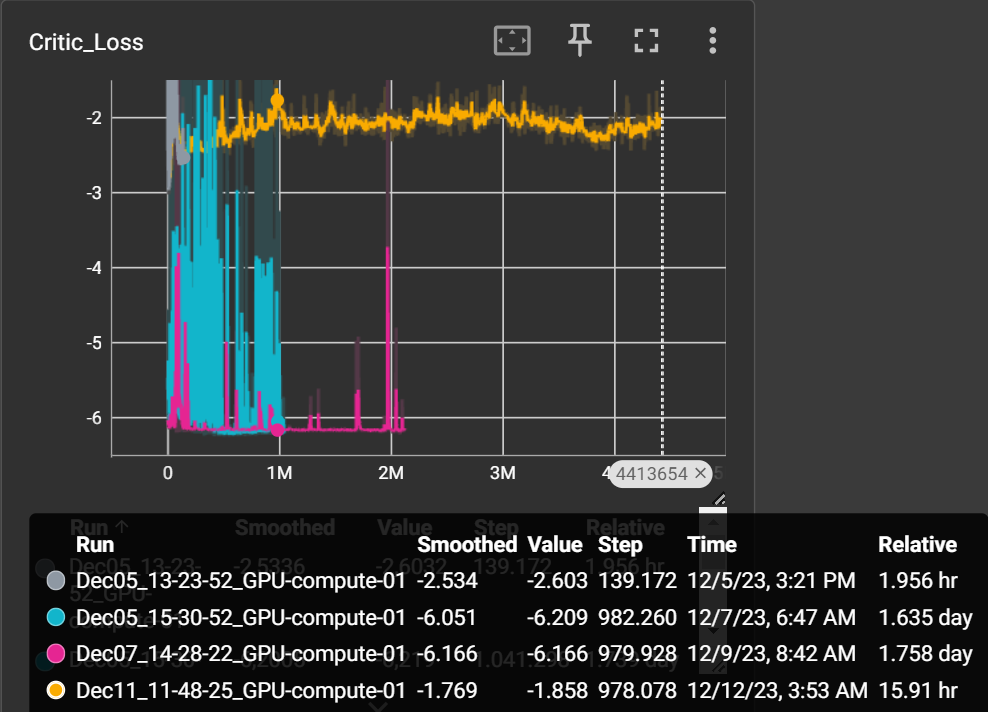
\includegraphics[height=5cm, keepaspectratio]{./img/alle_modelle.png}
\caption{Critic-Loss von den 4 verschiedenen langen Trainingverläufen}
\label{fig:critic_loss}
\end{minipage}
\hfill % Fügt einen horizontalen Zwischenraum ein
% Zweites Bild
\begin{minipage}[t]{0.45\textwidth}
\centering
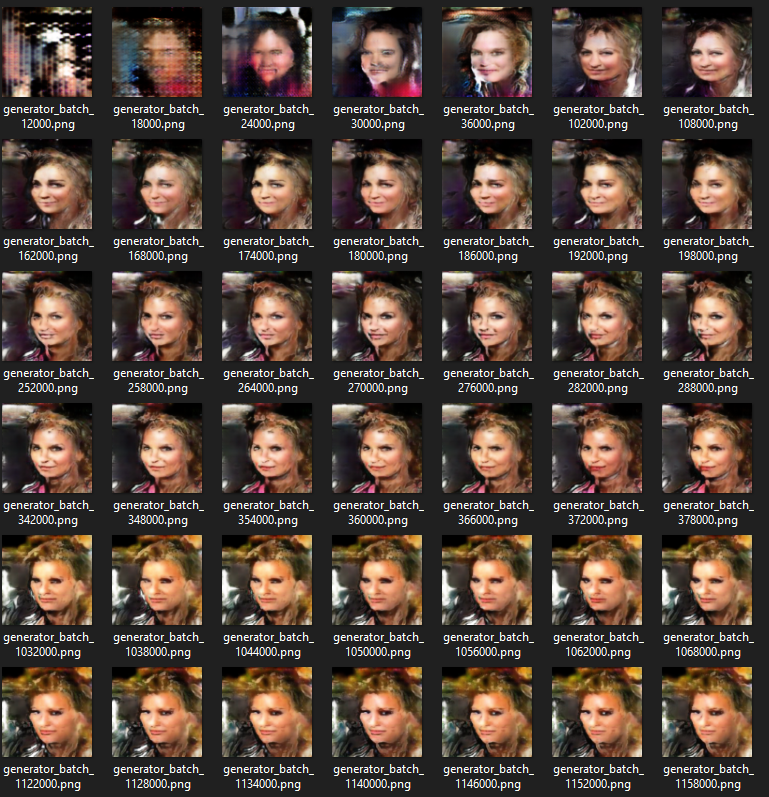
\includegraphics[height=5cm, keepaspectratio]{./img/epochs.png}
\caption{Das Modell mit der orangefarbenen Linie wurde für weitere Trainingsprozesse ausgewählt.}
\label{fig:epochs}
\end{minipage}
\end{figure}

\subsubsection{Increasing Image Resolution}
Encouraged by these improvements, I decided to gradually increase the resolution of the generated images, first to 128x128, then to 256x256 and 512x512 pixels. However, I encountered new challenges. Initially, training with higher resolutions did not work at all, which later turned out to be due to an unsuitable architecture. After spending weeks on unsuccessful training attempts, I finally managed to adjust the architecture and successfully train images at higher resolutions.

\subsubsection{Unexpected Results and Decisions}
During the training attempts with 256x256 and 512x512 pixels, I received unexpected results. The generated

 images sometimes showed more than one face, indicating the limited capabilities of WGANs at higher resolutions. For this reason, I decided to stay with a resolution of 128x128 pixels, as it provided more reliable and better-quality results.

Training with a resolution of 256x256 pixels generated images that led to unexpected representations with multiple faces, as seen in Figure \ref{fig:multiple_faces}. This phenomenon underscored the limited ability of WGANs to work effectively at higher resolutions.

This training process of the WGAN model was an intensive learning experience. It showed me the importance of careful review and adjustment of the model architecture and the challenges that arise when training GANs with increasingly higher resolutions.

\begin{figure}[ht]
\centering
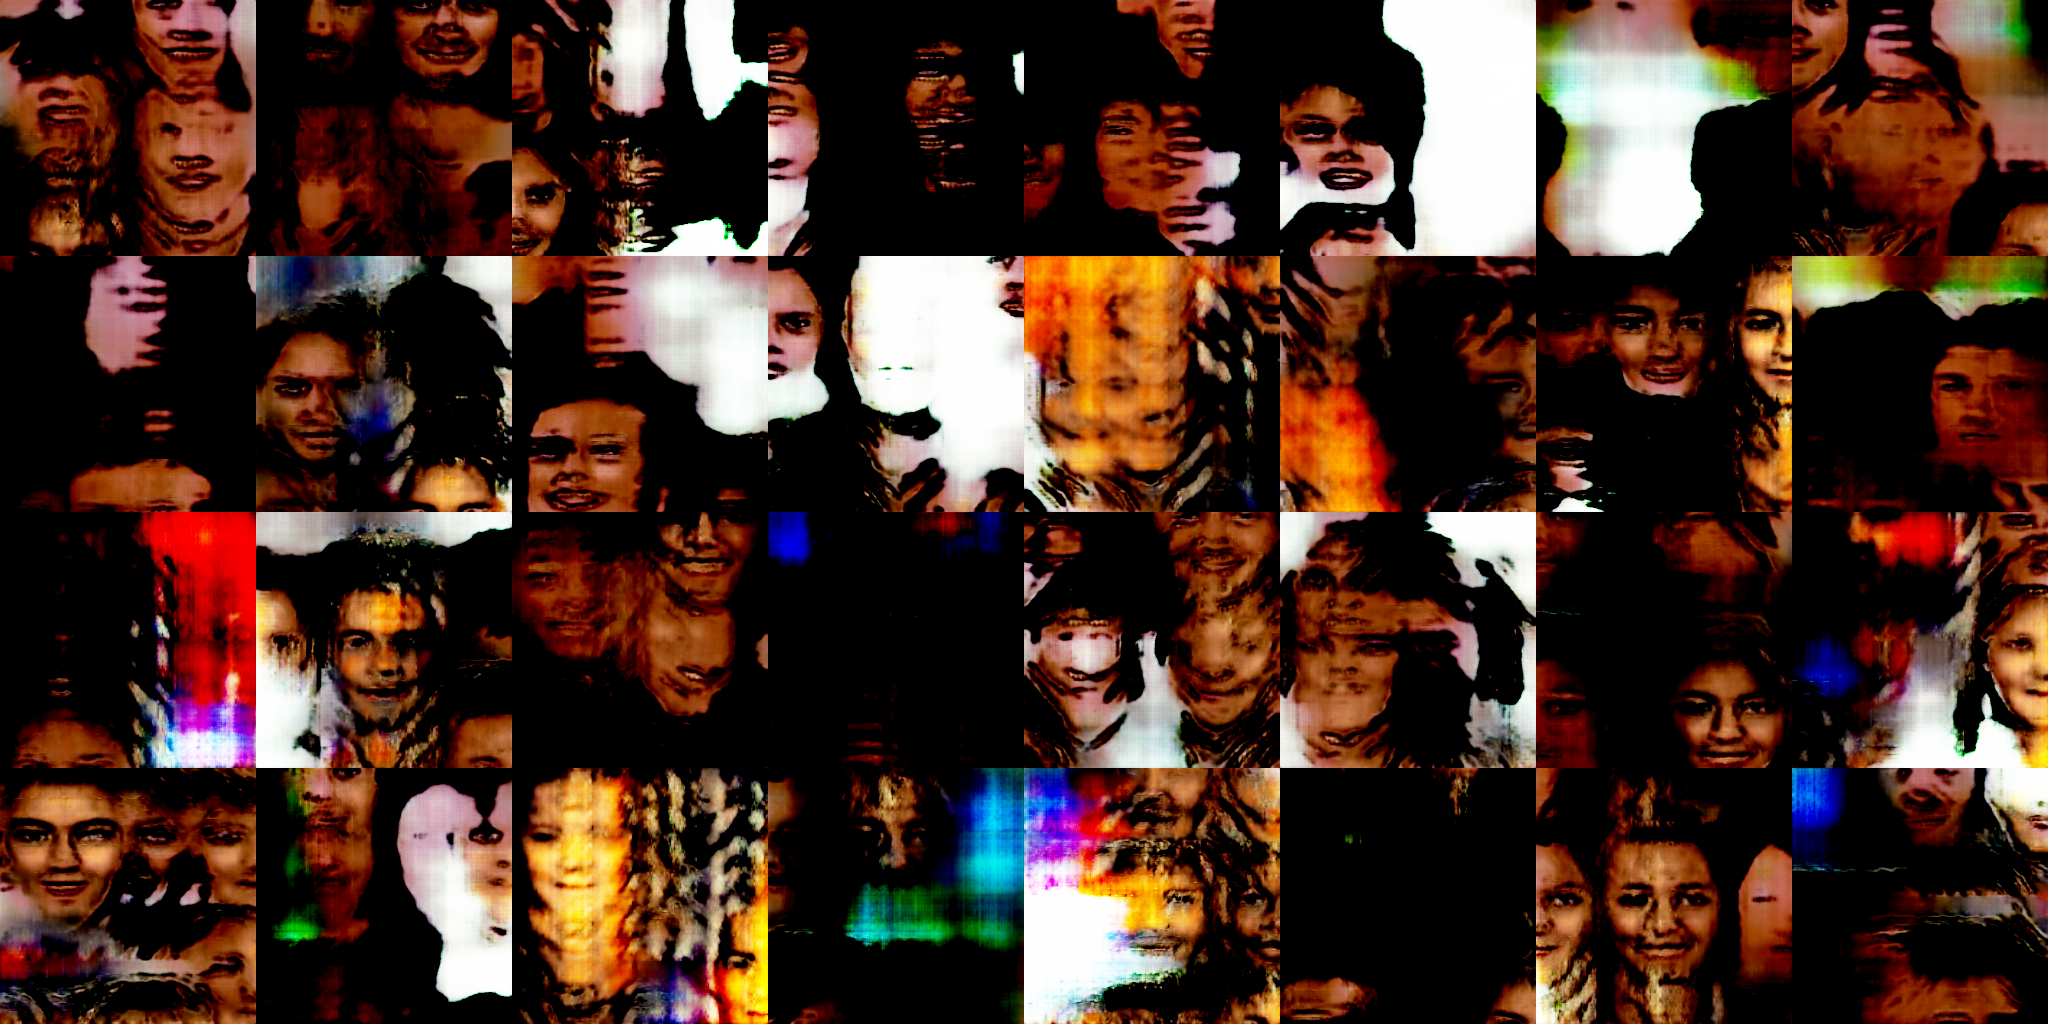
\includegraphics[width=0.8\textwidth]{./img/256x256.png}
\caption{At a resolution of 256x256 pixels, generated images with multiple face representations.}
\label{fig:multiple_faces}
\end{figure}

Given these results, I decided to limit the image resolution to 128x128 pixels, which led to better stability of the model and more reliable results. These experiences were essential for understanding the behavior and limitations of WGANs in image generation.
He

\section{Implementation}
\subsection{Generation of Latent Vectors and Interpolation}
The generation of latent vectors were key aspects of my WGAN project. These vectors form the basis for the generator to create diverse and realistic images.

\subsubsection{Generation of Latent Vectors}
The latent vectors, serving as input for the generator, were generated by producing random numbers using the torch.randn function in PyTorch. This method generates a tensor with normally distributed random numbers. I chose a vector size of 100 (nz), as this provides sufficient variety for generating different images. Each of these vectors represents a point in the latent space used by the generator to produce a unique image.

\subsubsection{Interpolation Between Vectors}
Interpolating between two latent vectors allows for smooth transitions between different generated images. For this purpose, I implemented linear interpolation (Lerp). Although initially planned to use spherical linear interpolation (Slerp), I limited myself to the simpler linear interpolation due to time constraints. This method calculates an intermediate vector by linearly combining the two end vectors. The combination ratio is gradually changed to produce a sequence of intermediate images that represent a smooth transition between the images generated by the generator.

This technique proved effective for creating a visually appealing sequence of transformations between two images, which was particularly useful for creating GIFs. Despite the relative simplicity of linear interpolation, it still offered the opportunity to explore and demonstrate the dynamics and potential of the latent space in the generated images.

\section{Results}
In my project, I created six GIFs, which are presented on the Readme page and stored in the "bests" folder. These visualizations show what is possible with the developed models. To further share the results, I uploaded the initial model and four additional models to Google OneDrive. By executing the command \texttt{python download\_model.py}, these models can be downloaded, allowing anyone to generate their own GIFs and fully explore the project.

\section{Next Steps}
The next steps include improving the transitions in the latent space by using slerp instead of lerp, leading to more natural transitions between generated images. Additionally, we aim to increase the quality and size of the images through two main strategies: either by further developing our own GAN network or by adapting a pre-trained model. Advanced techniques such as Progressive Growing of GANs, which gradually increases resolution, and Self-Attention GANs, which consider the relationships between parts of an image, will play a role. Both approaches require careful fine-tuning and testing to achieve optimal results.

\section{Summary and Outlook}
In my project, I experienced firsthand the fascination and challenges of Generative Adversarial Networks (GANs) by developing a GAN network completely from scratch. This experience allowed me to dive deeply into the mechanisms and potentials of this technology.

Dealing with the technical challenges, especially when scaling image resolution, has provided valuable insights into optimizing and adjusting GANs. These experiences lay a solid foundation for future projects and research in this area.

In conclusion, I look back with pride on what has been achieved. Although there are already more advanced models in this rapidly advancing field, this project has laid a solid foundation for my understanding of GANs. The experience of building a GAN network from scratch remains an unforgettable milestone in my academic and professional development.

\section{Bibliography}
\bibliographystyle{plain}
\bibliography{literatur}
\end{document}